%CLASSE DOCUMENTO - LINGUA E DIMENSIONE FONT
\documentclass[trieste,corpo=11pt,numerazioneromana]{toptesi}

%%%%%%%%%%%%%%%%%%%%%%%%%%%%%%%%%%%%%%%%%%%%%%%%%%%%%%%%%%%%%%%

% INCLUSIONE PACCHETTI
\usepackage[classica]{topfront}
\usepackage[utf8]{inputenc} %utf8
\usepackage[italian]{babel}
\usepackage[T1]{fontenc}
\usepackage{blindtext}
\usepackage{graphicx,wrapfig}
\usepackage{booktabs}
\usepackage{lmodern}
\usepackage{varioref}
\usepackage{epigraph}
\usepackage{url}
\usepackage{array}
\usepackage{paralist}{\obeyspaces\global\let =\space}
\usepackage{verbatim}
\usepackage{subfig}
\usepackage{tabularx}
\usepackage{amsmath}
\usepackage{amsfonts}
\usepackage{float}
\usepackage{float}
\usepackage{amssymb}
\usepackage{multicol}
\usepackage{multirow}
\usepackage{tabularx}
\usepackage{listings}
\usepackage[pass]{geometry}
\usepackage[figuresright]{rotating}
\usepackage{algorithm}
\usepackage{algorithmic}
\usepackage{wrapfig}
\usepackage{amsmath}
\usepackage[babel]{csquotes}
\usepackage{hyperref}
\usepackage{minted}
\usepackage[htt]{hyphenat}
\usepackage[backend=biber,bibencoding=ascii]{biblatex}

%%%%%%%%%%%%%%%%%%%%%%%%%%%%%%%%%%%%%%%%%%%%%%%%%%%%%%%%%%%%%%%

% CONFIGURAZIONE LINK E RIFERIMENTI
\hypersetup{%
    pdfpagemode={UseOutlines},
    bookmarksopen,
    pdfstartview={FitH},
    colorlinks,
    linkcolor={black}, %COLORE DEI RIFERIMENTI AL TESTO
    citecolor={blue}, %COLORE DEI RIFERIMENTI ALLE CITAZIONI
    urlcolor={blue} %COLORI DEGLI URL
}

%%%%%%%%%%%%%%%%%%%%%%%%%%%%%%%%%%%%%%%%%%%%%%%%%%%%%%%%%%%%%%%

% CONFIGURAZIONE LISTATI/CODICE - CANCELLARE SE NON NECESSARIO
% PYTHON - BIANCO E NERO
\lstset{%
	captionpos=b,
	language=Python,
	basicstyle =\small\ttfamily,
	keywordstyle=\color{black}\bfseries,
	breaklines=true,
	breakatwhitespace=true,
	frame=lines,
	numbers=left,
	numberstyle=\footnotesize,
}

%%%%%%%%%%%%%%%%%%%%%%%%%%%%%%%%%%%%%%%%%%%%%%%%%%%%%%%%%%%%%%%

% FRENCHSPACING VA _SEMPRE_ ABILITATO PER DOCUMENTI IN ITALIANO
\frenchspacing

%%%%%%%%%%%%%%%%%%%%%%%%%%%%%%%%%%%%%%%%%%%%%%%%%%%%%%%%%%%%%%%

%DEFINIZIONE SEZIONI IN NUMERAZIONE ROMANA
%ELENCO DEI LISTATI/CODICI
\makeatletter
\newcommand\listofcodes{%
 \iffrontmatter\else\frontmattertrue\fi
 \if@openright\cleardoublepage\else\clearpage\fi
 % change the meaning of \chapter in a group
 \begingroup\def\chapter##1{\@schapter}
 \phantomsection % for the hyperlink
 \addcontentsline{toc}{chapter}{Elenco dei listati}
 \lstlistoflistings
 \endgroup
}
\makeatother

\addto\captionsitalian{%
  \renewcommand{\lstlistlistingname}{Elenco dei listati}%
  \renewcommand{\lstlistingname}{Listato}%
}

%%%%%%%%%%%%%%%%%%%%%%%%%%%%%%%%%%%%%%%%%%%%%%%%%%%%%%%%%%%%%%%

% INFORMAZIONI PDF - PERSONALIZZARE
\pdfinfo{%
  /Title    (Realizzazione di un assistente vocale per il triage ospedaliero)
  /Author   (Simone Montali)
  /Subject  (Triage semi-automatizzato per la sicurezza e la tempestività)
  /Keywords (Triage ML Mycroft Ospedale Hospital)
}

%%%%%%%%%%%%%%%%%%%%%%%%%%%%%%%%%%%%%%%%%%%%%%%%%%%%%%%%%%%%%%%

% LISTA DEI CAPITOLI DA INCLUDERE - PERSONALIZZARE
\includeonly{%
introduzione,%
stateofart,%
mycroft,%
skills,%
fallback,%
informations,%
applicabilita,%
conclusioni,%
}

% FILE DI BIBLIOGRAFIA
\addbibresource{bibliography.bib}

%%%%%%%%%%%%%%%%%%%%%%%%%%%%%%%%%%%%%%%%%%%%%%%%%%%%%%%%%%%%%%%

% INIZIO DOCUMENTO
\begin{document}

%%%%%%%%%%%%%%%%%%%%%%%%%%%%%%%%%%%%%%%%%%%%%%%%%%%%%%%%%%%%%%%

% FRONTESPIZIO - PERSONALIZZARE
% ELIMINATE LE VOCI CHE NON VI SERVONO

% UNIVERSITA - NOME
\ateneo{Università degli studi di Parma}

% FACOLTA - DICITURA - CANCELLARE O DECOMMENTARE
%\FacoltaDi{Faculty of}
% FACOLTA - NOME
\facolta{Ingegneria}

% CORSO DI LAUREA - DICITURA (MANTENERE LO SPAZIO) - CANCELLARE O DECOMMENTARE
%\CorsoDiLaureaIn{Master of Science in }
% CORSO DI LAUREA - NOME
\corsodilaurea{Ingegneria dei Sistemi Informativi}

% TIPOLOGIA TESI
\TesiDiLaurea{Tesi di Laurea di primo livello}

% TITOLO
\titolo{Realizzazione di un assistente vocale per il triage ospedaliero}

% SOTTOTITOLO
\sottotitolo{Triage semi-automatizzato per la sicurezza e la tempestività}

% RELATORE/I - DICITURA - CANCELLARE SE UN SOLO RELATORE
\AdvisorName{Relatori}
% RELATORE - PROF. NOME E COGNOME
\relatore{prof.ssa\ Mordonini Monica}
% RELATORE AGGIUNTIVO - PROF NOME E COGNOME
% SE SI HA SOLO UN RELATORE ELIMINARE INSIEME AD AdvisorName
\terzorelatore{prof.\ Tomaiuolo Michele}
%\terzorelatore{prof.\ Angiani Giulio}
% CANDIDATO - DICITURA (MANTENERE I DUE PUNTI) - CANCELLARE O DECOMMENTARE
%\CandidateName{Candidate:}

% CANDIDATO - NOME E COGNOME
\candidato{Simone Montali}[288144]

% LOGO UNIVERSITA
\logosede{images/logo}

% DATA - MESE ANNO
\sedutadilaurea{Probabilmente 2020}

\frontespizio

%%%%%%%%%%%%%%%%%%%%%%%%%%%%%%%%%%%%%%%%%%%%%%%%%%%%%%%%%%%%%%%

%INTERLINEA - DEFAULT 1 - NON ESAGERATE, NON SUPERATE MAI 1.3 ;)
%\interlinea{1.2}

%%%%%%%%%%%%%%%%%%%%%%%%%%%%%%%%%%%%%%%%%%%%%%%%%%%%%%%%%%%%%%%

\frontmatter

% DEDICA - PERSONALIZZARE
% VSPACE - PROPORZIONE USATA PER CENTRATURA VERTICALE DEL TESTO
% FLUSHRIGHT - ALLINEAMENTO ORIZZONTALE A DESTRA
\vspace*{\stretch{1}}
\begin{flushright}
  \noindent
  Dedica toccante.
\end{flushright}
\vspace*{\stretch{6}}
\cleardoublepage


% CITAZIONE - PERSONALIZZARE
% VSPACE - PROPORZIONE USATA PER CENTRATURA VERTICALE DEL TESTO
% FLUSHRIGHT - ALLINEAMENTO ORIZZONTALE A DESTRA
\vspace*{\stretch{1}}
\begin{flushright}
  \noindent
  Citatemi dicendo che sono stato citato male.

  \textit{Groucho Marx}
\end{flushright}
\vspace*{\stretch{6}}
\cleardoublepage

%%%%%%%%%%%%%%%%%%%%%%%%%%%%%%%%%%%%%%%%%%%%%%%%%%%%%%%%%%%%%%%

% RINGRAZIAMENTI - PERSONALIZZARE
\ringraziamenti
Grazie

%%%%%%%%%%%%%%%%%%%%%%%%%%%%%%%%%%%%%%%%%%%%%%%%%%%%%%%%%%%%%%%

% ABSTRACT - PERSONALIZZARE
\sommario
Abstract della tesi
%%%%%%%%%%%%%%%%%%%%%%%%%%%%%%%%%%%%%%%%%%%%%%%%%%%%%%%%%%%%%%%

% INDICI - ELIMINARE GLI INDICI NON NECESSARI

% INDICE GENERALE
\tableofcontents

% INDICE DELLE FIGURE
\listoffigures

% INDICE DELLE TABELLE
%\listoftables

% INDICE DEI CODICI
%\listofcodes

%%%%%%%%%%%%%%%%%%%%%%%%%%%%%%%%%%%%%%%%%%%%%%%%%%%%%%%%%%%%%%%

\mainmatter

% INCLUSIONE FILE CAPITOLI - PERSONALIZZARE - TENERE COERENTE CON LISTA IN ALTO
\chapter{Introduzione}
\label{chap:introduzione}
In una società sempre più digitalizzata e dinamica, spesso viene a crearsi un netto distacco tra i settori capaci di \textbf{evolvere assieme alla tecnologia}, e quelli che, per un motivo o per l'altro, rimangono ancorati a procedure e metodologie tradizionali. Il settore medico, in continuo rinnovamento sul lato scientifico, è, soprattutto in Italia, affidato ad \textbf{infrastrutture informatiche progettate tempo fa.} Questo, soprattutto per motivi di stabilità e affidabilità: gli errori, qui, non sono ammissibili. \\
Per questo motivo, spesso non si notano le evidenti possibilità di miglioramenti che la ricerca informatica potrebbe apportare agli ospedali, agli ambulatori, agli studi.
L'obiettivo di questa tesi è mettere luce su una delle possibili modalità con cui l'informatica potrebbe, in un futuro prossimo, migliorare la praticità ma soprattutto la sicurezza degli ambienti ospedalieri.\\
La procedura di triage, ossia il processo di selezione dei pazienti richiedenti cure, è oggi affidata totalmente ad infermieri. Questa scelta è dovuta, oltre ad un evidente bisogno di poter osservare il paziente, alla necessità dell'\textbf{immediatezza di un contatto verbale} con il personale sanitario. \\
Perciò, la sfida nella realizzazione della tesi è soprattutto legata al rendere il \textbf{più umana possibile} l'interazione con un bot automatizzato. Il bot deve quindi accogliere il paziente, comprenderne le problematiche ed i sintomi, e farlo sentire protetto. Non si escluderà del tutto un apporto umano: gli infermieri sono addestrati per poter osservare e comprendere il richiedente cura, e l'apporto dell'osservazione diretta del paziente è ancora troppo importante per escluderla. È senz'altro possibile, però, affidare la prima parte di \textbf{profilazione dell'utente} a procedure automatizzate.

\chapter{Stato dell'arte}
\label{chap:stateofart}
Impara l'arte e mettila da parte.

\chapter{Mycroft}
\label{chap:mycroft}
\epigraph{There’s an entire community of developers looking to access this technology, but so far, it’s been the purview of a few large companies. The technology is walled-off, proprietary, and secretive.}{\textit{Joshua Montgomery \\ CEO di Mycroft AI, Inc.}}
Nel panorama degli assistenti vocali disponibili al pubblico, le grandi aziende catturano la maggior parte delle attenzioni dei consumatori. I nomi di Amazon Alexa, Google Home, Microsoft Cortana sono familiari a tanti. Meno familiare, però, è lo scenario degli stessi strumenti in ambito di assistenti vocali. Piattaforme come \textit{Jarvis}, \textit{Linto}, \textit{Open Assistant} e \textbf{Mycroft} sono sconosciute ai più. Quest'ultimo, negli ultimi anni, ha catturato l'attenzione di molti esperti di settore per la sua stabilità, espansibilità, popolarità.
\section{Open source}
\subsection{Cosa si intende con open source?}
Il termine \textbf{open source} si riferisce a qualcosa di modificabile e condivisibile dalle persone, avente quindi un \textbf{design pubblicamente accessibile.} Il termine nacque nell'ambito dello sviluppo software, ma oggi rappresenta, piuttosto, un'etica. Il software open source è software il cui codice sorgente è ispezionabile, modificabile, e migliorabile da chiunque voglia farlo. Con \textit{codice sorgente} intendiamo il codice che definisce il comportamento del programma, ossia il prodotto del lavoro di un programmatore. \\
Molti dei software che oggi utilizziamo sono invece \textbf{closed source} (o \textit{proprietario}), ossia software il cui codice sorgente non è accessibile agli utenti, e sul quale l'organizzazione che crea il software ha \textit{pieni poteri}. Alcuni esempi di software proprietario possono essere Windows, Photoshop, Safari. Solitamente, durante l'installazione di uno di questi software, l'utente accetta dei termini e condizioni che lo vincolano a non fare nulla di non autorizzato dall'azienda creatrice del software.
\subsection{Perché open source?}
Le motivazioni per preferire software open source rispetto a quelli proprietari sono svariate. Sebbene i software proprietari spesso abbiano funzionalità più avanzate e, spesso, meglio sviluppate, hanno gravi mancanze in progetti come questo. Il software open source, a scapito della possibilità di minori funzionalità (nonostante ciò non sia sempre vero, basti pensare alla potenza del kernel Linux), dà ad un utente esperto tante possibilità:
\begin{itemize}
    \item Possibilità di \textbf{controllo} sul software: la modifica e il miglioramento del software è permessa e ben vista. La comunità open source lavora con coesione per produrre software sempre migliore.
    \item Possibilità di conoscere e studiare i \textbf{meccanismi interni}: l'utilizzo di software per fini scientifici richiede la piena conoscenza di come un software funziona. Inoltre, la disponibilità del codice a tutti permette agli studenti e agli interessati di scoprire le logiche che ne permettono il corretto funzionamento.
    \item Grandi garanzie di \textbf{sicurezza}: se tutti possono accedere al codice, la presenza di bug di sicurezza e problematiche di privacy viene rilevata molto più velocemente di come accade nel software proprietario.
    \item Certezze sulla \textbf{privacy}: la società in cui viviamo è sempre più basata sulla vendita di dati personali acquisiti tramite software. L'open source, spesso e volentieri, si oppone a tale tendenza: essendo software della comunità e non di un'azienda che punta all'ottenimento di capitale, nessuno ha interesse nel \textit{monetizzare gli utenti}.
    \item Supporto della \textbf{comunità}: lo sviluppo di software open source è molto supportato dalla comunità informatica. In caso di problematiche o necessità, ci sarà sempre un utente più esperto disposto ad aiutare.
    \item Correttezza \textbf{etica}: software come quello oggetto di questa tesi hanno l'obiettivo di salvare vite. È giusto che tutti possano accedervi, migliorarlo e conoscerlo. La ricerca scientifica dovrebbe essere il più possibile \textbf{libera}.
\end{itemize}
\section{Introduzione a Mycroft}
Mycroft nacque tramite crowdfunding nel 2015 e catturò subito molto interesse da parte della comunità informatica. L'obiettivo era chiaro: opporsi alla sola presenza di software proprietario nel campo degli assistenti vocali. Ricevette presto l'appoggio di molte organizzazioni come la Canonical (promotrice di Ubuntu) e la Mozilla Foundation. La repository su Github di Mycroft conta oggi \textit{4300 stars} in continua crescita.
\subsection{Stack di funzionamento}
Come spiegato nel capitolo \ref{section:vocal_assistants}, un assistente vocale si compone principalmente di:
\subsubsection{Rilevamento della wake word}
L'assistente ha bisogno di rilevare una parola per attivarsi. Gli esempi più famosi sono \textit{Hey, Google} o \textit{Alexa}. Mycroft permette di personalizzare la propria wake word, che all'installazione è semplicemente \textit{Hey, Mycroft}. Il progetto utilizza \textbf{Precise}, un wake word listener basato su reti neurali addestrate su esempi audio. Questo componente, totalmente open source, è basato su \textit{pattern sonori}, non sul testo. La caratteristica ne riduce la dipendenza da accenti e linguaggi diversi. Precise offre la possibilità di addestrare il listener su un proprio dataset. Il funzionamento è basato su una singola rete neurale ricorrente, più precisamente una \textbf{Gated Recurrent Unit} o GRU.
\begin{figure}[H]
    \begin{center}
        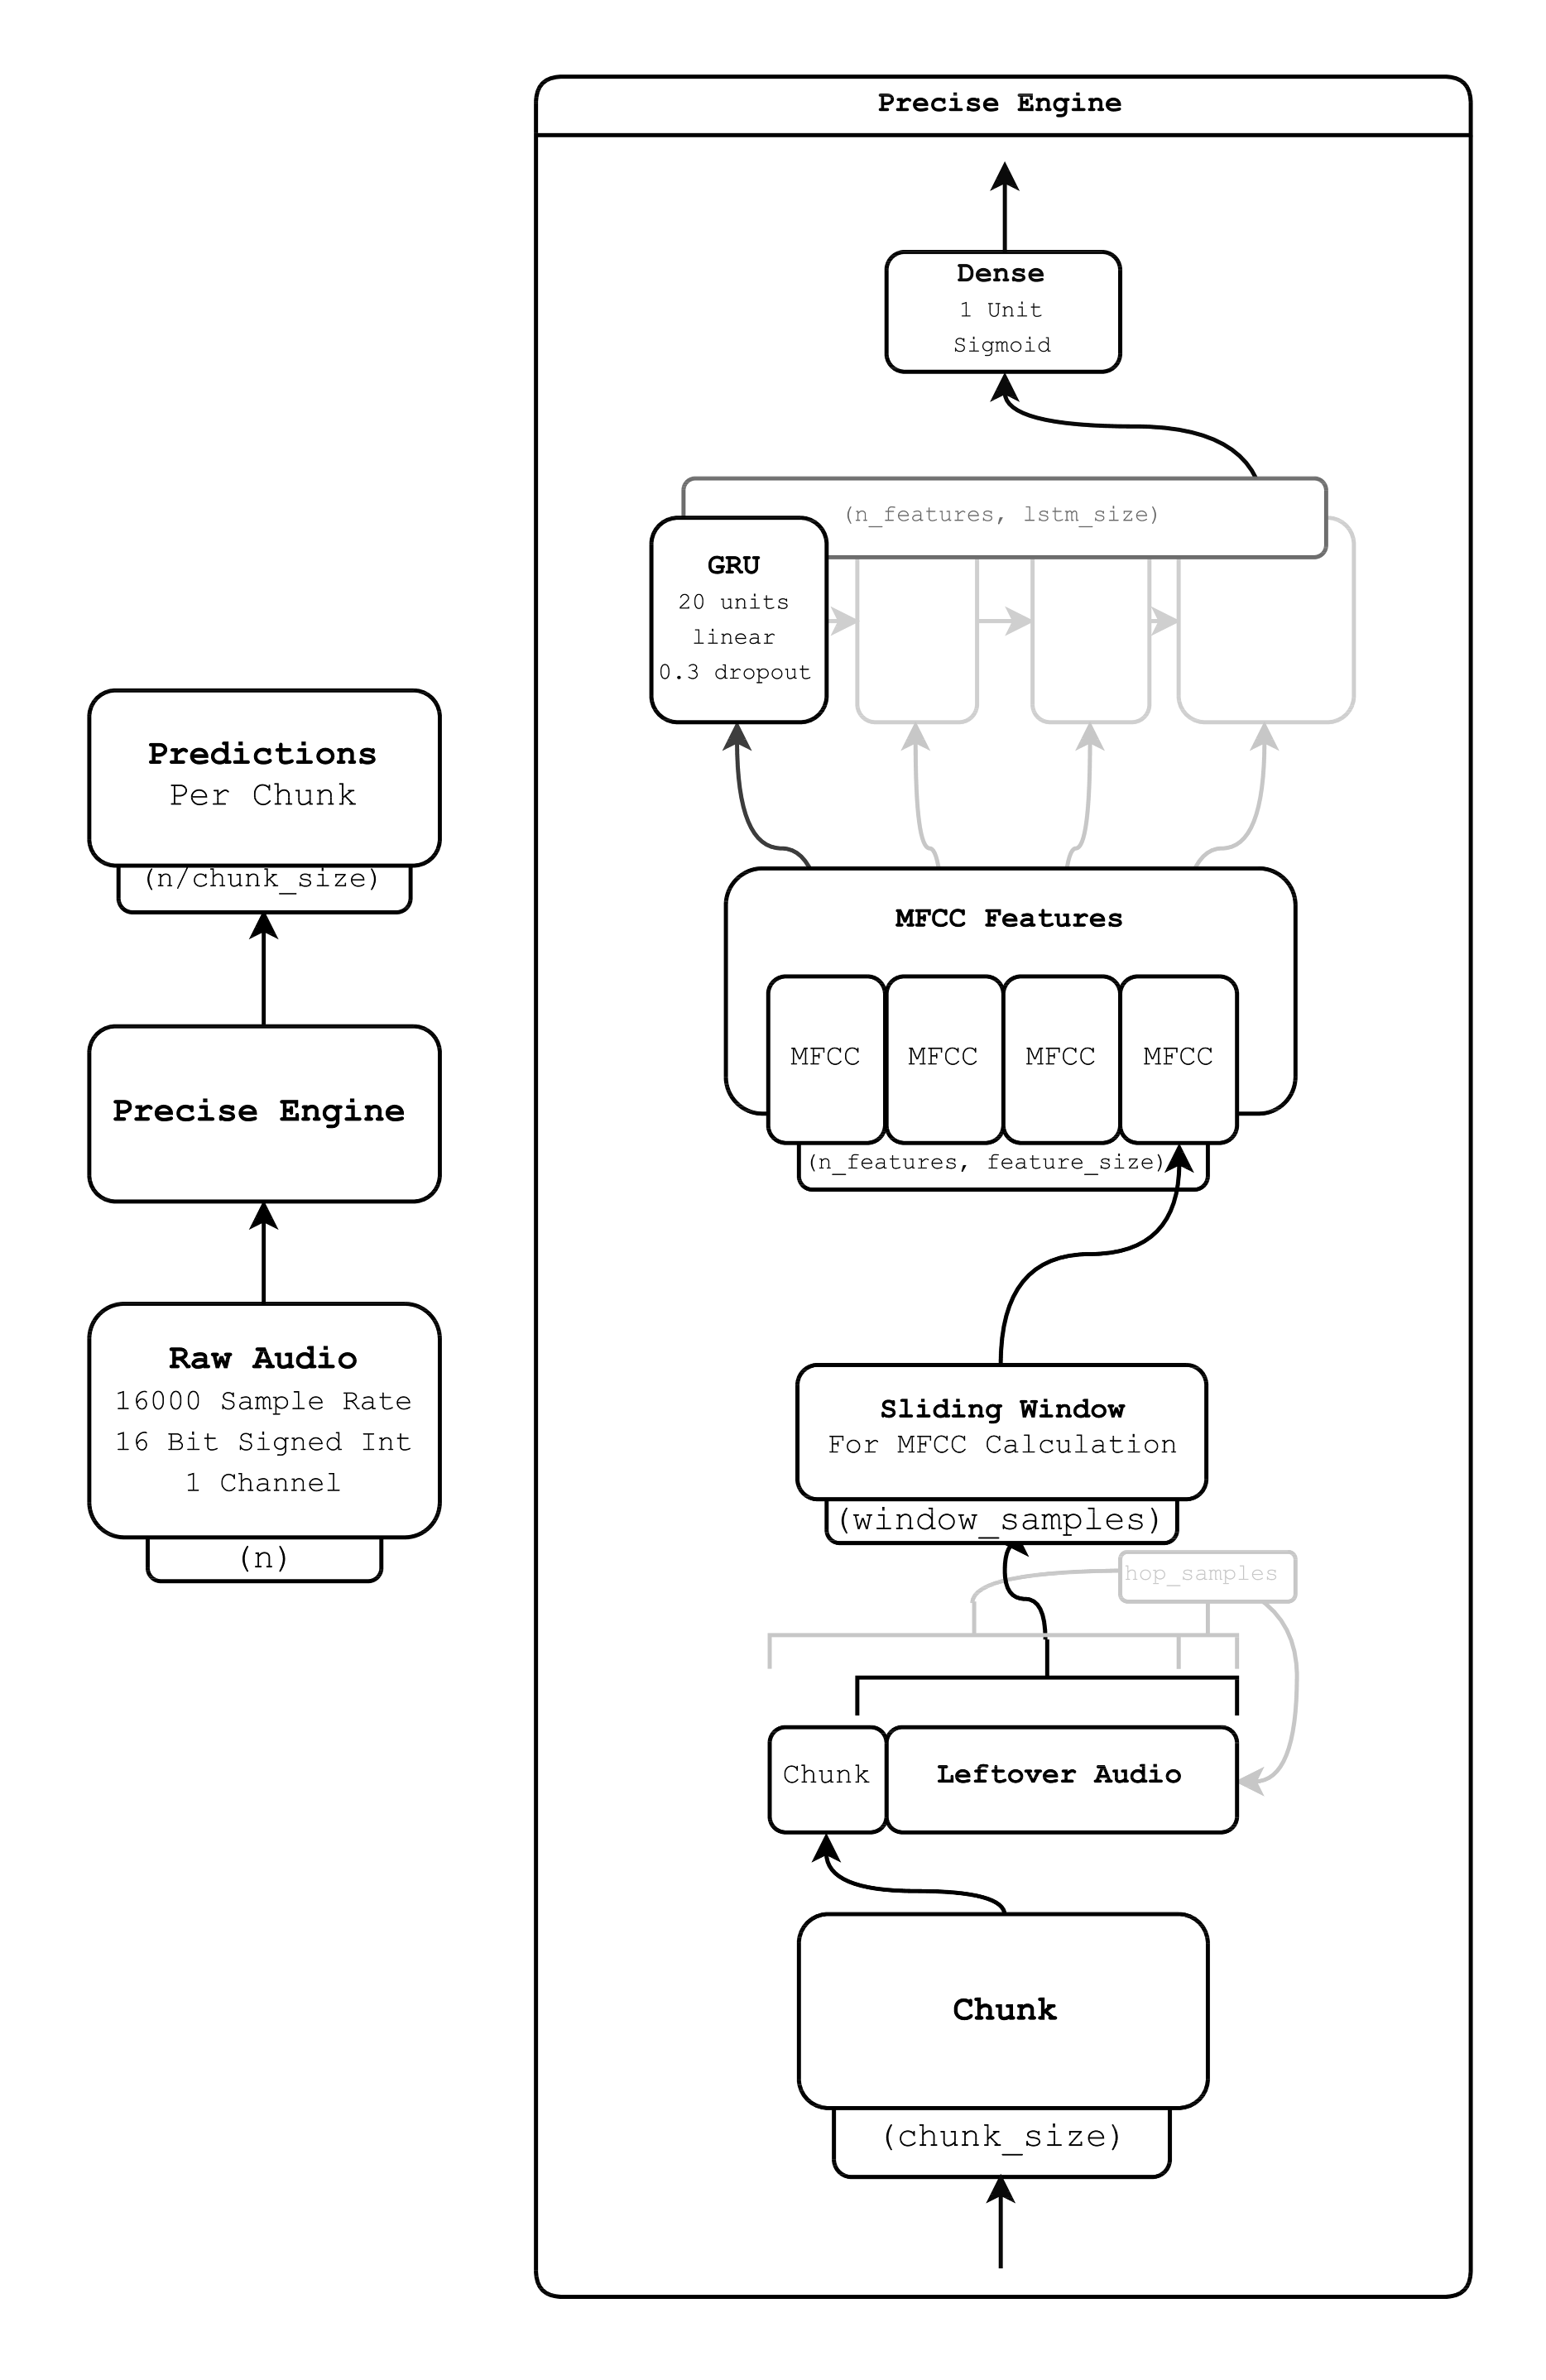
\includegraphics[width=0.6\columnwidth]{images/mycroft/precise.png}
    \end{center}
    \caption{Schema di funzionamento di Precise}
    \label{fig:precise}
\end{figure}
\subsubsection{Speech To Text}
Mycroft sfrutta il motore STT di Google per effettuare questo processo. Per aggiungere uno strato di privacy a queste richieste, esse vengono fatte passare attraverso i server Mycroft: Google non può ricollegare una richiesta all'utente che l'ha fatta. In questo modo, tutte le query effettuate a Google contengono solamente l'audio e hanno lo stesso mittente. In futuro sarà possibile sfruttare il dataset di \textbf{Mozilla Deepspeech}, che non è, ad oggi, ancora sufficientemente affidabile.
\subsubsection{Interpretazione degli intent}
Nell'ambito della speech recognition, un intent è l'operazione che l'utente \textit{intende} svolgere. Un utente può richiedere un'operazione in modi molto diversi. Lo scopo dell'intent parser è proprio quello di riuscire a superare questo scoglio, estraendo dalla richiesta scritta gli elementi chiave. Per esempio, se avessimo una richiesta del tipo "Hey Mycroft, domani pioverà a Parma?", l'intent parser dovrebbe capire:
\begin{itemize}
    \item L'utente desidera conoscere il \textbf{tempo atmosferico}.
    \item Il tempo atmosferico deve essere cercato per \textbf{Parma}.
    \item La data di interesse è \textbf{domani}.
\end{itemize}
Mycroft rende disponibili due software per la rilevazione di intenti: Padatious e Adapt. Mentre il secondo è basato sul riconoscimento di parole chiave, ed è quindi molto suscettibile alle richieste, il primo è composto da una rete neurale addestrata su frasi intere. Nel corso del progetto sfrutteremo \textbf{Padatious}.
Questo motore permette di avere creazione semplice degli intent, quantità di dati relativamente bassa, estrazione delle \textit{entities} semplice, addestramento rapido.
\subsubsection{Text To Speech}
Il componente di Text To Speech ha il compito di generare una traccia audio partendo dal testo di risposta codificato nella skill. Mycroft rende disponibile il progetto \textbf{Mimic}, basato sul software FLITE dell'università Carnegie Mellon. Purtroppo quest'ultimo non è disponibile in italiano, quindi nel corso del progetto utilizzeremo il motore TTS di Google, ottimizzato per l'italiano. Come sempre, le richieste passano attraverso i server Mycroft per ottenere un buon livello di privacy.
I testi di risposta sono codificati nei file vocabolario delle skills.
\subsection{Interfaccia grafica}
I dispositivi più avanzati di Mycroft come il \textit{Mark II} forniscono la possibilità di aggiungere interazioni visive con gli utenti. L'interfaccia è gestita da Mycroft-GUI, un componente aggiuntivo del bot che sfrutta i KDE Plasmoids, oggetti dell'interfaccia grafica KDE Plasma, simili a widget. La tecnologia è basata sul linguaggio QML, che permette una totale libertà nella creazione di interfacce, ma anche dei template standard semplici e rapidi da implementare. QML fa parte dello stack di tecnologie di Qt, una libreria multipiattaforma per lo sviluppo di programmi con interfaccia grafica.
\chapter{Realizzazione di skills}
\label{chap:skills}
Mycroft permette di espandere le abilità del bot in maniera semplice: è infatti costruito modularmente, ed è in ogni momento possibile espandere o ridurre i moduli attivi.
Questi moduli sono detti \textbf{skills}. Ogni skill è responsabile di una funzionalità: avremo ad esempio la skill del meteo, la skill che racconta barzellette o la skill che si occupa della domotica. Alla ricezione di una richiesta, Mycroft verifica gli intent e le keywords di ogni skill, attivando quella giusta.
% TODO: flowchart con adapt+padatious
La creazione di nuove skills è possibile grazie alla classe Python \texttt{MycroftSkill}, tramite la cui espansione possiamo definire i comportamenti della skill. All'installazione di Mycroft verrà reso disponibile il \textbf{Mycroft Skills Kit}, una command line interface che permette di eseguire le operazioni fondamentali collegate alle skills Mycroft. Tramite il comando \texttt{mycroft-msk create} verrà avviata una CLI che, dopo aver richiesto al programmatore alcune informazioni, genera il \textit{boilerplate code} necessario alla realizzazione della skill. Tra le informazioni richieste avremo nome, frasi d'esempio, dialoghi di risposta, descrizioni, etc\dots
Il template viene inoltre fornito di \texttt{git}, un sistema di versioning che permette di tenere traccia delle modifiche al codice e semplificare l'interazione tra programmatori.
\section{Struttura dei file della skill}
La struttura delle skills è ben organizzata, e vi sono diverse tipologie di file. Oltre a licenza e README, abbiamo tre componenti fondamentali per il funzionamento.
% TODO: dirtree
\paragraph{Directory \texttt{locale}}
Questa directory contiene i file dipendenti dalla lingua. Le sottocartelle seguono i tag linguistici IETF, quindi l'italiano sarà rappresentato da \texttt{it-it} e l'inglese (americano) da \texttt{en-us}. All'interno di queste, possiamo incontrare quattro tipologie di file:
\begin{itemize}
    \item \textbf{\texttt{dialog}}: questi file contengono i dialoghi di risposta del bot. Sono presenti più frasi simili, in modo da avere interazioni più "umane" con il bot, che sceglie una frase casuale tra queste. Ad esempio, \texttt{get\_age.dialog} conterrà le frasi \textit{"Mi potresti dire quanti anni hai?"}, \textit{"Per favore, dimmi la tua età"}, \textit{"Qual è la tua età?"}...
    \item \textbf{\texttt{intent}}: questi file contengono le frasi utilizzate per addestrare la rete neurale di Padatious. Ovviamente, più esempi vengono fatti, meglio la rete funzionerà. Per esempio, il file \texttt{symptoms.bleeding.intent} conterrà frasi come \textit{"Ho un'emorragia"}, \textit{"Sto sanguinando molto"}, \textit{"Ho una grande perdita di sangue"}...
    \item \textbf{\texttt{voc}}: questi file contengono keywords utilizzate in Adapt e nelle domande a risposta chiusa. Siccome il progetto si basa fortemente su Padatious, troviamo solo i file vocabolario per le domande sì/no ed il riconoscimento di numeri. Ad esempio, il file \texttt{yes.voc} conterrà \textit{"Sì"}, \textit{"Certo"}, \textit{"Esatto"}...
    \item \textbf{\texttt{entity}}: questi file contengono entità da estrarre negli intent. Ad esempio, l'intent \textit{fratture} estrae l'arto coinvolto nella frattura. Il file \texttt{limb.entity} conterrà quindi termini come \textit{"gamba"}, \textit{"pollice"}, \textit{"spalla"}...
\end{itemize}
\paragraph{\texttt{settingsmeta.yaml}}
Questo file contiene la definizione di impostazioni modificabili dall'utente sul sito di gestione di Mycroft. Ad esempio, l'utente potrebbe voler impostare i comportamenti di default, il nome del file esportato dal bot, una chiave API per l'integrazione con altri tool.
\paragraph{\texttt{\_\_init\_\_.py}}
Questo è il file principale della skill. Contiene il codice che definisce i comportamenti della skill. Il funzionamento è basato sull'espansione della classe \texttt{MycroftSkill}, che contiene i decorator ed i metodi necessari alla gestione della skill. Il prossimo capitolo si occuperà di definire la realizzazione vera e propria.
\section{Funzionamento della skill}
Tutta la realizzazione della skill è articolata intorno alla classe \texttt{MycroftSkill}.
\begin{minted}{python}
"""Mycroft skill that does a pre-triage on hospital patients.

The skill tries to ask the patient its symptoms, its personal data, 
and more. Then, it assigns a color code, stating a priority for
medical interventions.
"""

from mycroft import MycroftSkill, intent_file_handler
import json

class HospitalTriage(MycroftSkill):
    """Main skill class for the triage.

    This is the main skill class (extending MycroftSkill),
    which contains all the operations we need to perform the
    triage.

    Attributes:
        med_record: a dict containing all the patient data.
    """

    def __init__(self):
        MycroftSkill.__init__(self)
        self.med_record = {}
\end{minted}
\subsection{Metodi relativi alle sintomatologie}
La skill è stata strutturata come segue: ogni tipologia di sintomi equivale ad un intent, ed è quindi gestita da un metodo specifico. In base alla tipologia di sintomo, l'interazione viene poi gestita in modalità diverse: verrà assegnato al paziente un codice di triage, viene confermata al paziente la corretta comprensione del sintomo, viene mostrata sulla GUI l'informazione recepita. Terminate le operazioni specifiche del sintomo, le restanti procedure vengono gestite da decorators: la richiesta dell'anagrafica, dei sintomi minori, della febbre vengono eseguite indipendentemente dal problema riportato dal paziente. Un esempio di metodo relativo alle sintomatologie può essere il seguente:
\begin{minted}{python}
# BREATH
@intent_file_handler('symptoms.breath.intent')
@symptom_handler
@covid_symptom
def handle_breathing(self, message):
    """This function handles a "breathing fatigue" symptom.

    Breathing fatigue is recognized as a red code, and is a
    COVID-compatible symptom.

    Args:
        message: the message object returned from Mycroft

    GUI: show open mouth emoji
    """
    self.med_record["main_symptom"] = "breathing"
    self.med_record["code"] = "red"
    self.speak_dialog('symptoms.breath')
\end{minted}
Il metodo salva nell'oggetto \texttt{med\_record} (\textit{scheda clinica}) il sintomo principale, ossia problemi di respirazione, ed il codice relativo, in questo caso il rosso (accesso immediato alle cure). Poi, tramite il metodo \texttt{speak\_dialog} di \texttt{MycroftSkill}, pronuncia uno a caso tra i dialoghi contenuti nel file \texttt{symptoms.breath.dialog}, come
\begin{itemize}
    \item \textit{"Capisco, qualche problema di respirazione."}
    \item \textit{"Ok, segno nella scheda problemi di respirazione."}
    \item \textit{"Capito: problemi di respirazione."}
\end{itemize}
Da qui in poi, le operazioni sono affidate ai metodi chiamati dai decorators.
\subsection{Decorators utilizzati}
\subsubsection{Che cos'è un decorator?}
Anzitutto, occorre definire il comportamento di un decorator. Esso permette di assegnare responsabilità addizionali ad un oggetto, dinamicamente. Fornisce quindi un'alternativa flessibile al \textit{subclassing}. Definire un decorator in Python significa definire dei comportamenti da eseguire prima e dopo l'esecuzione del metodo vero e proprio.
\subsubsection{Applicazione del concetto al programma}
Alcune operazioni sono, all'interno del progetto, ricorrenti. Ad esempio, la richiesta di anagrafica o di sintomi minori deve essere fatta in tutti e soli i metodi relativi alla gestione di sintomi. Alcuni di questi (quelli compatibili con il COVID19, come la tosse), avranno bisogno inoltre di approfondimenti per valutare la possibilità che il paziente sia affetto da COVID19, facendogli domande specifiche. Sono stati quindi definiti due decorators aggiuntivi:
\paragraph{\texttt{symptom\_handler}} Questo metodo, dopo aver gestito le operazioni specifiche di un sintomo, prosegue con le procedure generali, come la richiesta dell'anagrafica, di una valutazione del dolore, di altri sintomi, e, per ultima, l'esportazione della cartella clinica.
\begin{minted}{python}
def symptom_handler(handler):
"""Decorates a symptom with the needed operations.

This function is used as a decorator for symptoms, adding
operations like personal data asking, age, other symptoms...

Returns:
    The decorator function
"""
def ask_about_symptoms(*args, **kwargs):
    returned = handler(*args, **kwargs)
    args[0].med_record["symptom_declaration"] = args[1].data["utterance"]
    # I'm using args[0] here instead of self, but it works the same
    args[0].request_age()
    args[0].request_other_symptoms()
    args[0].evaluate_pain()
    args[0].request_name()
    args[0].export_med_record()
    return returned
return ask_about_symptoms
\end{minted}
\paragraph{\texttt{covid\_symptom}} La situazione di emergenza che il mondo sta vivendo al momento della stesura di questa tesi ha richiesto particolare attenzione verso le sintomatologie compatibili con COVID19: distanziare i pazienti che potrebbero essere portatori di virus al più presto è la \textbf{sfida più grande del momento}. Per questo, il decorator, aggiunto ai soli sintomi compatibili con la malattia, permette di interrogare il paziente riguardo alcune caratteristiche tipiche della malattia, come il fiato corto, la difficoltà a percepire i sapori, la febbre alta.
\begin{minted}{python}
def covid_symptom(handler):
        """Decorates a COVID-compatible symptom.

        This function is used as a decorator in the COVID-compatible
        symptoms. It proceeds to ask the COVID-related questions
        to the patient.

        Returns:
            The decorator function
        """
        def check_if_covid(*args, **kwargs):
            returned = handler(*args, **kwargs)
            args[0].ask_covid_questions()
            return returned
        return check_if_covid
\end{minted}
Il metodo \texttt{ask\_covid\_questions} procede ad intervistare il paziente con il modello di diagnosi più usato al momento. Ogni domanda posta al paziente ha un suo \textit{score} caratteristico, che moltiplica un indice relativo al paziente in base alla gravità ed alla connessione con la malattia. Le caratteristiche indagate sono:
\begin{itemize}
    \item \textbf{Febbre}: moltiplicatore $2$
    \item \textbf{Mal di gola}: moltiplicatore $1.3$
    \item \textbf{Raffreddore}: moltiplicatore $1.3$
    \item \textbf{Fatica respiratoria}: moltiplicatore $1.6$
    \item \textbf{Tosse}: moltiplicatore $1.6$
    \item \textbf{Contatti con infetti}: moltiplicatore $2$
    \item \textbf{Mancanza di gusto}: moltiplicatore $1.7$
\end{itemize}
Ogni paziente sospetto ha inizialmente un \texttt{covid\_score} di $1$, che viene moltiplicato per i vari indici se il paziente risponde in modo affermativo. Se lo score supera una soglia predeterminata (al momento fissata a $15$), è sospetto COVID19 e verrà destinato ad un'area di triage apposita.
\begin{minted}{python}
def ask_covid_questions(self):
    """Checks for COVID symptoms.

    When triggered by a COVID-compatible symptom, 
    this function evaluates the patient symptoms to 
    try to guess if he/she has COVID19.

    GUI: show face mask emoji
    """
    self.speak_dialog('gotta_check_covid')
    covid_score = 1
    # Let's check if the patient knows the temperature. Skip if he already declared it.
    if not "fever" in self.med_record:
        self.check_fever()
    if "fever" in self.med_record:
        if self.med_record["fever"] > 37.5:
            covid_score = covid_score * 2
    # Let's define an array of tuples, each containing the yes/no question
    # string and its COVID index multiplier
    yesno_questions = [("has_sore_throat", 1.3), ("has_cold", 1.3),
     ("has_breathing_difficulties",1.6), ("has_cough", 1.6),
     ("has_had_contacts", 2), ("misses_taste", 1.7)]
    self.speak_dialog('will_ask_yesno')
    # Check if he/she has COVID-compatible symptoms
    for question in yesno_questions:
        self.med_record[question[0]] = self.ask_yesno(question[0])
        if self.med_record[question[0]] == 'yes':
            covid_score = covid_score * question[1]
        self.log.info(covid_score)

    self.med_record["covid_score"] = covid_score
    if covid_score > 15:
        self.speak_dialog('probably_has_covid')
    else:
        self.speak_dialog('doesnt_have_covid')
    self.log.info(self.med_record)
\end{minted}
\subsection{Helper methods}
Sono, oltre ai metodi caratteristici della classe, presenti alcuni \textit{helper methods} utili ad operazioni interne del software. Di seguito elenchiamo i più importanti:
\paragraph{\texttt{extract\_temperature}} Questo metodo, data una stringa in ingresso rappresentante la temperatura corporea che può essere in vari formati (ad esempio, il paziente potrebbe pronunciare \textit{"Trentasette e mezzo", "Trentasette virgola cinque", "Trentasette punto cinque", "Trentasette e cinque"} indicando sempre la stessa temperatura), la estrae in formato decimale.
\begin{minted}{python}
def extract_temperature(utterance):
    """Extracts the patient temperature from the utterance.

    This is needed because of the various ways of Mycroft interpreting
    floating point numbers. Some examples:
    - 38 e 1
    - 38/1
    - 38.1
    - 38,1
    - 38 1

    Returns:
        The floating point value of the temperature, or
        None if it is impossible to extract.
    """
    # Beware: the ' e ' has to be before the simple space!
    possible_separators = ['/', '.', ',', ' e ', ' ']
    try:
        for separator in possible_separators:
            if separator in utterance:
                temperature_strings = utterance.split(separator)
                if temperature_strings[1] == "mezzo":
                    temperature_strings[1] = "5"
                temperature = int(
                    temperature_strings[0])+float(temperature_strings[1])*0.1
                return temperature
        return None
    except TypeError:
        return None
\end{minted}
\paragraph{\texttt{age\_validator}} Questo metodo, fornito al metodo \texttt{get\_response}, definisce se un'età è valida. In caso negativo, viene chiesta nuovamente.
\paragraph{\texttt{number\_validator}} Questo metodo verifica se l'input vocale è numerico, distinguendo anche il caso in cui un \textit{sei} venga interpretato come \textit{verbo essere} e non $6$.
\subsection{Oggetto \texttt{med\_record}}
Tutti i dati della procedura di triage confluiscono in un oggetto \texttt{med\_record}, in cui vengono salvati per l'inserimento nel database ospedaliero. Questo oggetto verrà poi esportato in formato JSON (\textbf{J}ava\textbf{S}cript \textbf{O}bject \textbf{N}otation) con la possibilità di essere inviato ad un'API REST del sistema esistente.
\begin{minted}{python}
def export_med_record(self):
"""Exports the data to JSON.

This function is called at the end of the interaction
to export the fetched data from the patient. It then
assigns a desk to the patient based on his/her severeness.

GUI: show hands emoji
"""
with open("med_record.json", "w") as med_record_file:
    med_record_file.write(json.dumps(self.med_record))
self.speak_dialog('thanks_and_bye', {"desk": self.med_record["code"]})
self.med_record = {}
\end{minted}
Questo formato standard permette di essere integrato semplicemente con infrastrutture preesistenti. Per esempio, un paziente affetto da COVID19 potrebbe avere la seguente scheda clinica:
\inputminted{json}{code/med_record.json}
\chapter{Fallback skills e NLP}
\label{chap:fallback}
Sorge, dopo il lavoro svolto fino ad ora, un dubbio: cosa accadrebbe se la richiesta del paziente non fosse tra quelle previste durante la realizzazione della skill?
Le necessità mediche delle persone sono, purtroppo, ben più vaste di quanto si possa pensare di programmare. Viene quindi utile un approccio più "statistico", applicabile grazie alle più recenti scoperte nell'ambito dell'intelligenza artificiale.
\section{Classificazione del testo}
Esiste, nell'intelligenza artificiale, una branca che si occupa di \textbf{Natural Language Processing}, ossia processamento del linguaggio naturale. Vorremo quindi trovare un \textit{sistema} che approssimi al meglio la corrispondenza tra un input testuale ed un output che indichi una specifica classe. Il processo sarà quindi diviso in più parti: per primo, dovremo trovare un dataset testuale già categorizzato, o categorizzarne manualmente uno. Fatto ciò, dovremo trovare un modo di poter addestrare il computer a riconoscere i \textit{pattern} che legano un determinato testo alla sua classe d'appartenenza.
\section{Dataset utilizzato}
La presenza in rete di siti web come \textit{Kaggle} semplifica nettamente la ricerca di un dataset adatto alle necessità del data analyst. Purtroppo le moderne normative sulla privacy impongono la totale riservatezza dei dati medici delle persone. Esistono però, fortunatamente, dei dataset creati ad-hoc per la risoluzione di problematiche come quella qui presentata. Il dataset sfruttato per questa tesi\cite{dataset:medical-speech}, creato dalla \textbf{Appen}, azienda australiana specializzata in \textit{training data}, contiene audio, trascrizioni e intents di pazienti richiedenti aiuto. Tutto il dataset è in lingua inglese. Siccome la parte di Speech To Text viene gestita da Mycroft, utilizzeremo soltanto il dataset di trascrizioni ed intents. Ad esempio, alcune entries del dataset, potrebbero essere:
\begin{table}[H]
    \begin{tabularx}{\textwidth}{|l|X|}
        phrase: & My son had his lip pierced and it is swollen and the skin inside on his lip is grey and looks infected.
        \\
        prompt: & Infected wound
    \end{tabularx}
\end{table}
\begin{table}[H]
    \begin{tabularx}{\textwidth}{|l|X|}
        phrase: & I used to be out of breath after going up a dozen of stairs, but now I struggle to breath even when I sit down.
        \\
        prompt: & Hard to breath
    \end{tabularx}
\end{table}
\subsection{Traduzione del dataset}
\label{section:traduzione}
Siccome il bot deve funzionare anche in italiano, risulta evidente la necessità di una traduzione. Potremmo pensare di utilizzare le API di Google Translate, ma la traduzione di tutti i record del dataset (circa 8000), avrebbe un prezzo non indifferente. Si potrebbe quindi risolvere automatizzando l'utilizzo dell'interfaccia web tramite uno strumento come \textit{Selenium}. Fortunatamente, esistono già librerie Python per fare esattamente questo. Tra queste, \textbf{googletrans} è la più supportata dalla comunità.
Questa permette di definire un oggetto \texttt{Translator()} che sfruttiamo per la traduzione:
\begin{minted}{python}
for index, row in data.iterrows():
    phrase = translator.translate(row["phrase"], dest="it").text
    prompt = translator.translate(row["prompt"], dest="it").text
    if translator.detect(phrase).lang == "it" and translator.detect(prompt).lang == "it":
        translated_data.at[i, "phrase"] = phrase
        translated_data.at[i, "prompt"] = prompt
        i = i+1
\end{minted}
Quando Google Translate non riconosce il significato di una frase, non la traduce e la lascia come l'originale.
Notiamo che l'oggetto \texttt{translator} permette, oltre alla traduzione, di rilevare la lingua di una stringa. Questa caratteristica è d'aiuto per la realizzazione di un piccolo \textit{workaround} alle mancate traduzioni: se la funzione \texttt{detect} non rileva la lingua italiana sia nel testo che nella classe di appartenenza, la riga viene saltata. Questo riduce il numero di entries da circa 8000 a poco più di 2000. Gli esempi prima riportati sono ora:
\begin{table}[H]
    \begin{tabularx}{\textwidth}{|l|X|}
        phrase: & Mio figlio ha avuto il labbro trafitto ed è gonfio e la pelle all'interno del suo labbro è grigia e sembra infetta.
        \\
        prompt: & Ferita infetta
    \end{tabularx}
\end{table}
Notiamo qui che un piercing è diventato un \textit{labbro trafitto}, ma il senso generale è comunque ben chiaro.
\begin{table}[H]
    \begin{tabularx}{\textwidth}{|l|X|}
        phrase: & Ero senza fiato dopo aver salito una dozzina di scale, ma ora faccio fatica a respirare anche quando mi siedo.
        \\
        prompt: & Difficile da respirare
    \end{tabularx}
\end{table}
Anche qui, notiamo un piccolo problema di traduzione: le classi come \textit{"breathing difficulties"} vengono tradotte in modo letterale. Essendo però le classi in numero limitato, possiamo effettuare un \textit{find and replace}, passando, ad esempio, a \textit{Difficoltà respiratorie}.
\section{Addestramento della rete neurale}
Avendo ora un dataset in italiano, possiamo procedere con l'addestramento di una rete neurale che classifichi i testi. Per fare ciò, si è deciso di sfruttare la libreria \textbf{fastai}.
\subsection{fastai}
La libreria \textbf{fastai} semplifica il training e la creazione di reti neurali tramite le più recenti scoperte nell'ambito del deep learning. Tra le varie interfacce disponibili nella libreria, siamo interessati alla sezione riguardante il testo. Qui, è presente la classe \texttt{text.learner}, il cui scopo principale è addestrare un modello tramite il metodo \texttt{fit()}. Questa libreria permette inoltre di esportare suddetto modello, allo scopo di integrarlo in applicazioni senza dover effettuare il training ad ogni utilizzo. Esattamente quello che fa al nostro caso: possiamo addestrare la rete neurale una volta sola, ed utilizzare i risultati dell'addestramento a tempo indeterminato nell'assistente vocale, sostituendoli solo quando migliorati.
\subsection{Preparazione dei dati}
Una volta ottenuto il file CSV tradotto, effettuiamo l'importazione su Google Colab e li inseriamo in un dataframe per verificare l'assenza di NaN. Fatto ciò, possiamo creare una \texttt{TextList} di \textit{fastai}. Questo oggetto è un'\texttt{ItemList} specializzata nel testo, ossia una struttura di memoria che raggruppa gli input per il modello.
\begin{minted}[]{python}
path = Path('/content/')
data_clas = (TextList.from_csv(path, 'translations.csv', 
                            cols='phrase')
                .random_split_by_pct(.2)
                .label_from_df(cols='prompt')
                .databunch(bs=42))
\end{minted}
Fatto ciò, creiamo l'oggetto \texttt{text\_classifier\_learner}. Questo è basato su una Recurrent Neural Network. Scegliamo, come architettura, \texttt{AWD-LSTM}, che si è dimostrata vincente nella risoluzione di problemi di classificazione del testo simili a questo. % TODO: Può convenire spiegarla meglio? https://yashuseth.blog/2018/09/12/awd-lstm-explanation-understanding-language-model/
Addestriamo quindi la rete, e generiamo una confusion matrix, che permette di verificare quanto errate siano le classificazioni, e quali errori sono più ricorrenti.
\begin{figure}[H]
    \begin{center}
        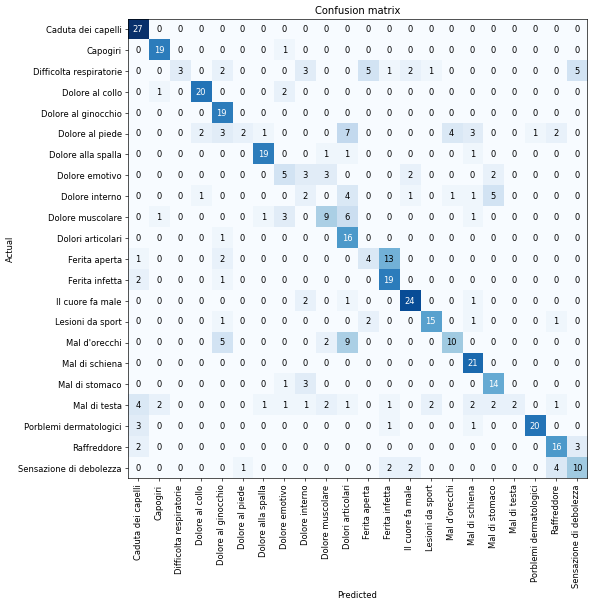
\includegraphics[width=0.8\columnwidth]{images/fallback/ConfusionMatrix.png}
    \end{center}
    \caption{Confusion Matrix}
    \label{fig:confusion-matrix}
\end{figure}
Notiamo il formarsi di una diagonale nella tabella: questo è sintomo di un \textbf{modello funzionante}. Possiamo quindi ora esportare il modello per l'utilizzo futuro.
\begin{minted}[]{python}
learn.export('/content/exported_model')
\end{minted}
\section{Realizzazione di fallback skills}
Come precedentemente spiegato, Mycroft funziona riconoscendo determinati \textit{intent} nelle richieste dell'utente. Questi sono stati da noi definiti nella skill del capitolo precedente. Abbiamo però specificato nell'introduzione che, a volte, i casi che abbiamo codificato non sono sufficienti:
\begin{enumerate}
    \item Svenimenti
    \item Emorragie
    \item Shock
    \item Difficoltà respiratorie
    \item Fratture
    \item Febbre
    \item Ustioni
    \item Dolori addominali
\end{enumerate}
Se si trattasse di una categoria esterna a queste, il paziente \textbf{non potrebbe venire aiutato}. Esiste però la possibilità di definire delle \textit{fallback skills}, ossia delle skill chiamate dall'assistente vocale quando la frase non viene riconosciuta dalle skill classiche. Queste hanno una priorità, e vengono chiamate nell'ordine definito da questa. Se una fallback skill riesce a risolvere la richiesta, non viene inoltrata alle altre. Vogliamo quindi ora creare un'automazione che sfrutti il modello ricavato dal natural language processing di cui sopra.
\subsection{Registrazione della skill}
La skill estende la classe \texttt{FallbackSkill}. Durante l'\textit{init} dell'oggetto, registriamo la fallback con una priorità di 10:
\begin{minted}[]{python}
self.register_fallback(self.handle_fallback, 10)
\end{minted}
Fatto ciò, possiamo caricare il modello di classificazione del testo precedentemente generato, assicurandoci che la libreria \textbf{fastai} sia installata.
\begin{minted}[]{python}
# Load the classifier model
self.learner = load_learner('models', 'exported_model')
# Load the classifier classes from JSON
with open('classes.json') as classes:
    self.classes = json.load(classes)
\end{minted}
Carichiamo inoltre il file \texttt{classes.json}, contenente le corrispondenze tra l'output numerico del modello e le classi testuali, oltre alle informazioni riguardanti la compatibilità del sintomo con il COVID19, l'immagine da mostrare nella GUI, e la gravità del sintomo:
\begin{minted}[]{json}
{
    "name": "Dolore al collo",
    "emoji": "[rimosso per motivi di stampa]",
    "code": "yellow",
    "covid": false
}
\end{minted}
Fatto ciò, resta da definire il comportamento del bot alla chiamata della fallback, operazione che svolgeremo con il metodo \texttt{handle\_fallback}.
Idealmente, questo dovrà predirre la classe del sintomo, chiederne conferma al paziente, e aggiungere le informazioni alla scheda di triage.
\begin{minted}[]{python}
@symptom_handler
def handle_fallback(self, message):
    utterance = message.data.get("utterance")
    symptom = self.classes[int(self.learner.predict(utterance)[0])]
    self.gui.show_text(symptom["emoji"])
    did_i_get_that = self.ask_yesno(
        'symptoms.fallback', {"symptom": symptom["name"]})
    if did_i_get_that == "no":
        self.speak_dialog('sorry')
    else:
        if symptom["covid"]:
            self.ask_covid_questions()
        self.med_record["main_symptom"] = symptom["name"]
        self.med_record["code"] = symptom["code"]
\end{minted}
Ora il nostro bot, in caso di mancato riconoscimento del sintomo, potrà comunque indirizzare il paziente in modo automatizzato.
\chapter{Richieste di informazioni da parte degli utenti}
\label{chap:informations}
I casi d'uso di uno strumento come questo assistente vocale potrebbero però \textbf{non fermarsi al mero indirizzamento di pazienti}. Infatti, potremmo plausibilmente aspettarci che gli utenti desiderino anche \textbf{ottenere informazioni di carattere medico} senza doversi per forza rivolgere ad un dottore.
\section{Enciclopedia medica del Ministero della Salute}
Pare ovvio sottolineare che le fonti delle informazioni riferite ai pazienti debbano essere \textbf{il più affidabili possibile}. Affidarsi a siti web come Wikipedia, per quanto comodo possa essere, è rischioso: le informazioni possono essere modificate da chiunque, anche e soprattutto persone poco qualificate.
Esiste però, in rete, una risorsa sconosciuta ai più, ma senz'altro interessante per i nostri scopi: l'\textbf{Enciclopedia Medica del Ministero della Salute}, accessibile sul sito del suddetto.
\begin{figure}[h]
    \begin{center}
        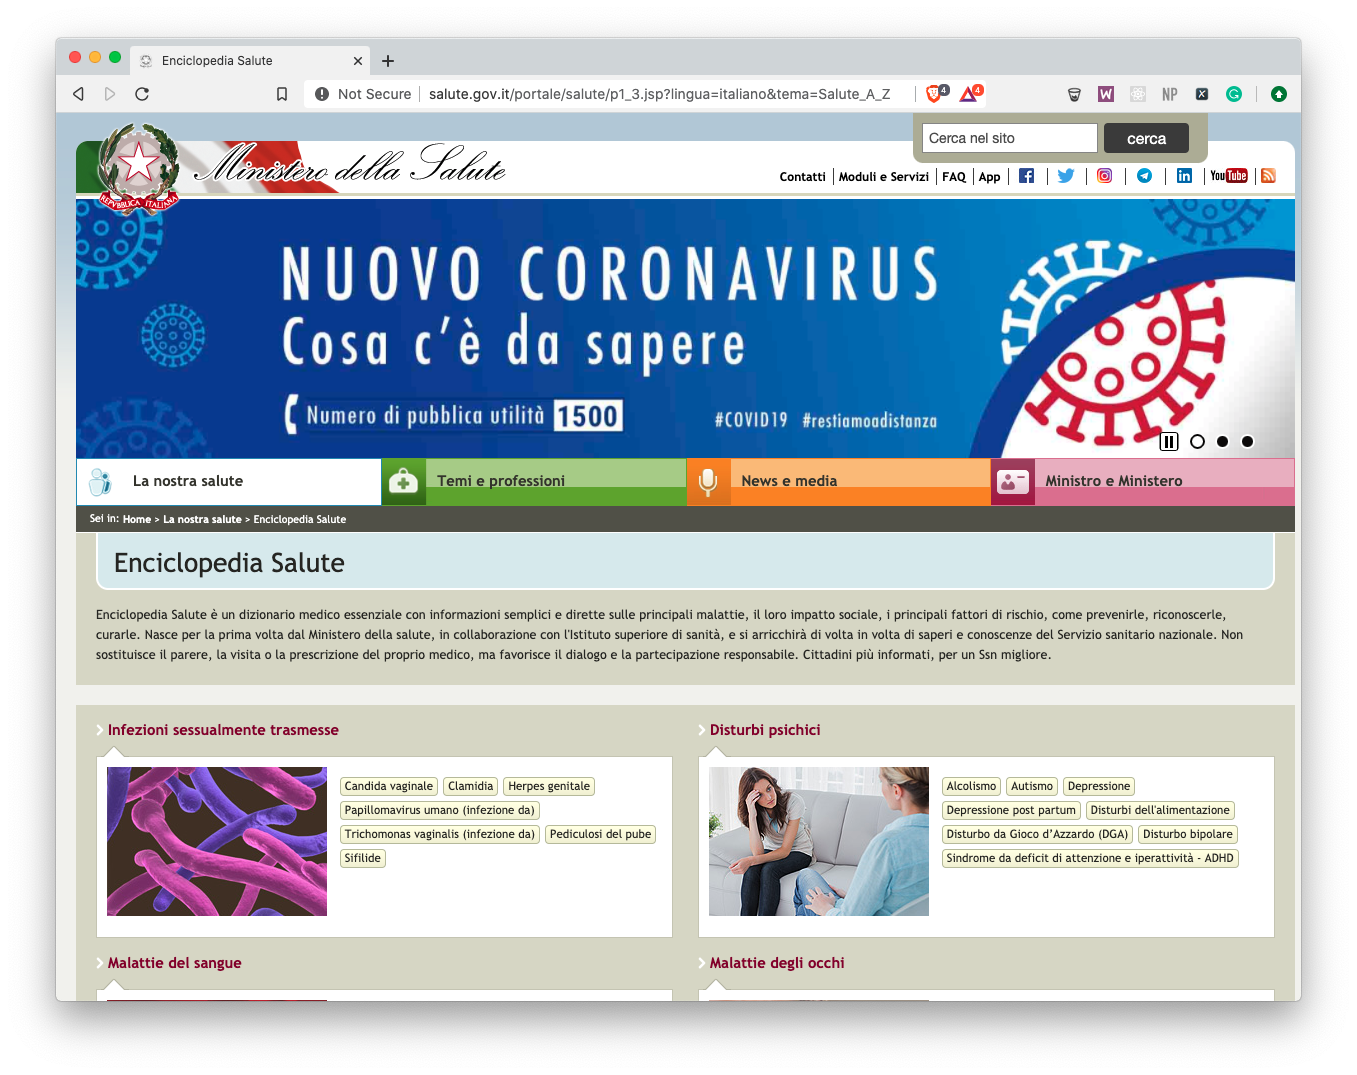
\includegraphics[width=0.8\columnwidth]{images/informations/MinSalute.png}
    \end{center}
    \caption{Enciclopedia della Salute}
    \label{fig:min-salute}
\end{figure}
\subsection{Utilizzo dell'enciclopedia}
Si potrebbe inizialmente pensare di trascrivere le informazioni dal sito: questo non è però certamente un approccio efficiente. Vorremmo allora automatizzare l'interazione con il sito web, in modo da ottenere i dati in modo autonomo. Viene, in nostro soccorso, il framework \textbf{Selenium}.
\subsubsection{Selenium}
Selenium è un framework nato con lo scopo di testare applicazioni web. È utilizzabile tramite un IDE proprietario, disponibile come estensione per Mozilla Firefox e Google Chrome, ma anche tramite scripts che interagiscono con \textbf{Selenium WebDriver}. Quest'ultimo accetta comandi in \textit{Selenese} o tramite una \textit{Client API}, e li trasmette ad un browser che ne raccoglie i risultati. È possibile definire questi scripts di testing in linguaggi diversi dal Selenese: dalla versione 2.0, Selenium WebDriver è totalmente implementato e supportato in Python, Ruby, Java e C\#. Durante il progetto abbiamo utilizzato la versione Python, installabile tramite PIP:
\begin{minted}[]{shell}
    pip3 install -U selenium
\end{minted}
Dopo l'installazione di Selenium, è ovviamente necessario anche un driver per interfacciarsi con il browser. Quello per Firefox è ad esempio \textit{GeckoDriver}, quello per Chrome \textit{ChromeDriver}. Ora, definire script per l'automazione di applicazioni web è semplice. Creando un oggetto tramite \texttt{webdriver.Firefox()}, avremo la possibilità di inviare comandi al browser ed interagire con la pagina web. Per fare ciò, ci basta selezionare un elemento tramite la sua classe CSS, il suo ID, un XPath: \texttt{find\_element\_by\_class\_name("nav-tabs")}. Fatto ciò, basta, ad esempio, chiamare il metodo \texttt{click()} sull'elemento. È anche possibile eseguire codice JavaScript: sul sito del Ministero della Salute, ad esempio, per disattivare il popup contenente le normative sui cookies sarà sufficiente eseguire \texttt{execute\_script("setPrivacy();")}.
\subsubsection{Approccio API}
Se i dati sul sito web cambiassero spesso, sarebbe molto utile definire un'API in modo da poter scaricare i dati al momento della richiesta. Tramite la libreria \texttt{http.server} è possibile definire una classe API (che estenda \texttt{BaseHTTPRequestHandler}), che ascolti una porta in attesa di richieste ed invii le risposte. Ad esempio, definendo un metodo \texttt{do\_GET}, esso verrà chiamato ogni qualvolta il server riceva una richiesta di tipo GET sulla porta designata. Definendo un oggetto \texttt{DataFetcher} che si occupi di gestire Selenium e l'interazione con la pagina, il metodo di risposta alla GET potrebbe essere così composto:
\begin{minted}[]{python}
def do_GET(self):
    parameters = parse_qs(urlparse(self.path).query)
    response = DataFetcher(parameters["query"][0])
    if response is not None:
        self.send_response(200)
    else:
        self.send_response(404)
    self.send_header('Content-type', 'application/json')
    self.send_header('Access-Control-Allow-Origin', '*')
    self.end_headers()
    if response is not None:
        self.wfile.write(json.dumps(response.get_query()).encode())
\end{minted}
Nella classe \texttt{DataFetcher}, dopo aver lanciato il WebDriver nell'\texttt{\_\_init\_\_}, basterà cercare il termine della query, e scorrere le tabs della pagina dell'enciclopedia. Essa è infatti divisa in sezioni come \textit{"Come si trasmette"}, \textit{"Sintomi"}, \textit{"Descrizione"}. Inviando quindi una richiesta tramite \textit{HTTPie}:
\begin{minted}[]{shell}
$ http "localhost:8000/?query=celiachia"

HTTP/1.0 200 OK
Access-Control-Allow-Origin: *
Content-type: application/json
Date: Fri, 19 Jun 2020 09:49:30 GMT
Server: BaseHTTP/0.6 Python/3.7.6

{
    "Cause": "La celiachia è una condizione multifattoriale, 
                [testo accorciato per motivi di stampa]",
    "Complicanze": "I soggetti affetti da celiachia non trattata 
                presentano un rischio maggiore di sviluppare complicanze, 
                [testo accorciato per motivi di stampa]",
    "Descrizione": "La celiachia, o malattia celiachia, è una malattia 
                permanente su base infiammatoria dell'intestino tenue caratterizzata 
                dalla distruzione della mucosa di questo tratto intestinale.
                [testo accorciato per motivi di stampa]",
    "Diagnosi": "Nei soggetti ad alto rischio di celiachia, per familiarità,
                 sintomi o per la presenza di una malattia frequentemente associata, 
                 [testo accorciato per motivi di stampa]",
    "Sintomi e segni": "I sintomi e segni della malattia sono estremamente
                 variabili per sede ed intensità.[testo accorciato per motivi di stampa]",
    "Terapia": "L’unica terapia attualmente disponibile per i soggetti celiaci
                 è la completa e permanente [testo accorciato per motivi di stampa]"
}
\end{minted}
\subsubsection{Approccio periodico}
Eseguire richieste all'API durante l'interazione con l'assistente vocale può generare \textbf{fastidiosi ritardi}. Siccome le informazioni sul sito web di cui sopra \textbf{non vengono aggiornate spesso}, può essere conveniente aggiornarle una volta al giorno e tenerle salvate in locale. Questo elimina del tutto i ritardi nel recupero delle informazioni, e ci permette un'integrazione \textbf{molto più efficace} in Mycroft: sapendo quali termini medici sono presenti nell'enciclopedia e quali no, il bot saprà già quali riconoscere e quali, invece, restituiranno un errore. Sfruttando come sempre Selenium, possiamo definire uno script utilizzando, in parte, il codice definito precedentemente. Basterà infatti chiamare la funzione \texttt{get\_query()} ciclicamente, una volta per termine disponibile nell'enciclopedia, ed accorpare tutti i risultati in un \textit{dictionary}, da salvare poi in JSON.
\begin{minted}[]{python}
def get_all(self):
    self.driver.get(MINISTERO_SALUTE_ENCYCLOPEDIA)
    fetched_data = {}
    aree = self.driver.find_elements_by_class_name("aree")
    for i in range(0, len(aree)):
        # This is kinda esoteric: the references on the DOM get changed on every refresh. 
        # So, we have to re-get them every time.
        aree = self.driver.find_elements_by_class_name("aree")
        aree[i].click()
        data = self.get_query()
        if data is not None:
            fetched_data[self.driver.title] = data
        self.driver.get(MINISTERO_SALUTE_ENCYCLOPEDIA)
    return fetched_data
\end{minted}
Una volta terminata l'esecuzione, ci basterà esportare i dati. Per fare ciò, utilizziamo due file: uno contenente le \textbf{informazioni}, uno contenente le \textbf{patologie conosciute}, da passare a Mycroft per il training di Padatious:
\begin{minted}[]{python}
data = df.get_all()
with open("informations.json", "w") as info_file:
    json.dump(data, info_file)
with open("locale/it-it/disease.entity", "w+") as entity_file:
    for name in data:
        entity_file.write(name+"\n")
\end{minted}
Fatto ciò, basterà definire un intent di Mycroft con frasi come \textit{"Dammi informazioni (sul|sulla|del|della|dei|sui) \{disease\}"}, dove \texttt{\{disease\}} indica un riferimento al file appena definito, contenente le malattie conosciute. È importante sottolineare come queste non siano strettamente richieste: un paziente potrebbe usare delle terminologie diverse. Per questo, vorremmo che il bot cercasse la malattia con \textbf{la miglior corrispondenza}, piuttosto che cercarla letteralmente. In questo modo, per esempio, "Tumore ai polmoni" sarebbe comunque ricollegabile a "Tumore del polmone". Una volta riconosciuta la malattia, Mycroft dovrà verificare \textbf{quali tipologie di informazioni possiede su di essa}, e chiedere all'utente di scegliere, domandando, ad esempio, \textit{"Cosa ti piacerebbe sapere? Scegli tra Sintomi, Cura, Terapia"}.
\begin{minted}[]{python}
# Let's find the most similar disease to what we've got
key, result = dictionary_searcher(
    message.data.get('disease'), self.informations)
# Tell the user the best match, and if it was wrong, say sorry
did_i_get_that = self.ask_yesno(
    "info.check_results", {"disease": key})
if did_i_get_that == "no":
    self.speak_dialog('sorry')
    return
# Let's create an array containing the choices of infos
self.possibilities = result
choices = ""
for choice in self.possibilities:
    choices = choices + choice + ", "
response = self.get_response(dialog='info.possibilities', data={
    "possibilities": choices})
info_key, info = dictionary_searcher(response, result)
self.speak_dialog(
    'info.speak', {"infos": info})
\end{minted}
Il bot è ora in grado di tenere conversazioni con i pazienti al riguardo di malattie, patologie, cure:
\begin{itemize}
    \item \textit{"Cosa sai dirmi sulla celiachia?"}
    \item \textit{"Ho trovato risultati per celiachia, è ciò che cercavi?"}
    \item \textit{"Esatto!"}
    \item \textit{"Cosa ti piacerebbe sapere? Scegli tra cause, complicanze, descrizione, diagnosi, sintomi e segni, terapia."}
    \item \textit{"Dimmi le cause."}
    \item \textit{"Ecco ciò che so: la celiachia è una condizione multifattoriale, [testo accorciato per motivi di stampa]"}
\end{itemize}
\section{Esempio di conversazione}
Riportiamo ora un esempio di conversazione realmente avvenuto.
\begin{itemize}
    \item \textbf{Utente:} \textit{Cosa sai dirmi sul tumore al fegato?}
    \item \textbf{Bot:} \textit{Il miglior risultato è Tumore del Fegato, è ciò che cercavi?}
    \item \textbf{Utente:} \textit{Esatto}
    \item \textbf{Bot:} \textit{Cosa ti piacerebbe sapere? Scegli tra Descrizione, Segni e sintomi, Cause, Diagnosi, Terapia, Prevenzione}
    \item \textbf{Utente:} \textit{Prevenzione}
    \item \textbf{Bot:} \textit{Questo è ciò che so: le uniche misure per ridurre le probabilità di ammalarsi di cancro al fegato sono l'adozione di stili di vita e misure di igiene che contrastino i fattori di rischio per questa forma tumorale}
\end{itemize}
\section{Aggiornamento dei dati}
Potrebbe configurarsi la necessità di verificare periodicamente il sito del Ministero della Salute in cerca di correzioni, modifiche, novità. Siccome la piattaforma è eseguita in ambienti Linux, uno straordinario strumento viene in nostro soccorso: \textbf{cron}. cron è un job scheduler per sistemi operativi UNIX. La sua struttura semplice permette di definire operazioni periodiche da svolgere in determinati istanti di tempo, all'interno di file detti \textbf{crontab} (\textit{cron table}). Ogni linea del crontab indica un'operazione da svolgere e gli istanti di tempo a cui farlo:
\begin{minted}[]{shell}
[min] [ore] [giorno] [mese] [giornodellasettimana] <comando da eseguire>
\end{minted}
Un asterisco sta ad indicare \textit{a tutti/e i/le ore/minuti/giorni...}. È anche possibile definire frazioni di intervalli di tempo: \texttt{*/2} verrà eseguito ad esempio una volta su due. Se quindi volessimo eseguire il fetching dei dati ogni notte, alle 02:00, basterebbe inserire nel crontab la seguente linea:
\begin{minted}[]{shell}
0 2 * * * cd hospital-triage-skill & python3 info_updater.py
\end{minted}
I più attenti potrebbero chiedersi perché non lanciare direttamente \texttt{python3 hospital-triage-skill/info\_updater.py}. Questo comando, apparentemente uguale al precedente, cela una grande differenza: non modifica la \textit{working directory} della linea di comando, che rimane la cartella home dell'utente. Essendo però i file salvati secondo un percorso relativo nel corso dello script Python, apparirebbero direttamente nella cartella home piuttosto che in quella del progetto.
\chapter{Applicabilità e requisiti tecnici}
\label{chap:applicabilita}
Resta ora da analizzare la fattibilità del progetto nel mondo reale. Questo assistente vocale potrebbe \textbf{migliorare ampiamente il workflow} di molte cliniche ospedaliere, anche all'estero. Infatti, eseguire la traduzione in un'altra lingua è un lavoro svolgibile da chiunque, trattandosi della mera traduzione di stringhe. Si potrebbe, addirittura, pensare di integrare il modulo Python \texttt{googletrans} citato in \ref{section:traduzione}, rendendo il progetto poliglotta.
\section{Requisiti tecnici}
Analizziamo i vari componenti dell'assistente vocale per comprenderne i requisiti tecnici:
\subsection{Text To Speech e Speech To Text}
Queste operazioni vengono svolte in cloud tramite le API di Google, e richiedono quindi \textbf{solamente una connessione ad internet}. Ovviamente, si configura la necessità di periferiche audio per la cattura e la riproduzione di audio. Un \textbf{microfono universale} ed un \textbf{set di altoparlanti} possono sopperire a tale necessità.
\subsection{Analisi degli intent}
L'assistente vocale procede all'analisi degli intent tramite Padatious e Adapt. Mentre il secondo si basa sul riconoscimento di hotwords, e non ha quindi grandi necessità in termini di calcolo, il primo è composto da una rete neurale che viene addestrata ad ogni avvio del bot. Questa è probabilmente l'\textbf{operazione che richiede più potenza} di calcolo. Tuttavia, essendo svolta al solo avvio del bot, basterebbe pensare di avviare il bot \textbf{qualche minuto prima} dell'effettiva necessità di utilizzo per risolvere questa problematica.
\subsection{fastai}
Essendo il training del modello svolto a priori, non avremo grandi necessità di potenza di calcolo: l'operazione di \textit{inference} è \textbf{molto più leggera} dell'addestramento. È suggeribile quindi eseguire quest'ultimo su un computer più potente o direttamente in cloud, con strumenti come Google Colab, per poi \textbf{esportare il modello} nel formato di fastai tramite il comando \texttt{learn.export('/content/exported\_model')}.
\subsection{Interfaccia grafica}
Il software \textbf{Mycroft GUI} fa un pesante utilizzo del framework Qt, più specificatamente dei KDE Plasmoids, componenti grafici (simili a widgets) che caratterizzano l'ambiente desktop KDE Plasma. Per questo, risulta ovvio che il dispositivo su cui viene eseguito l'assistente vocale debba essere compatibile con il suddetto. Il team di Mycroft suggerisce, come sistema operativo, \textbf{KDE neon}, consistente in una versione di  Ubuntu LTS con installato l'ambiente KDE Plasma. Questo nome garantisce un'ottima stabilità, semplicità d'uso, compatibilità.
\section{Compatibilità, dispositivi ottimali e costi}
La sezione precedente ha evidenziato come i requisiti tecnici dell'assistente vocale siano compatibili con una \textbf{vastissima gamma di dispositivi}, anche economici. Questo potrebbe \textbf{sgravare un'ulteriore spesa} ad un sistema ospedaliero vittima, da anni, di tagli e budget stringenti. Il software potrebbe infatti essere installato su un vecchio computer, o su un Raspberry Pi.
\begin{figure}[H]
    \begin{center}
        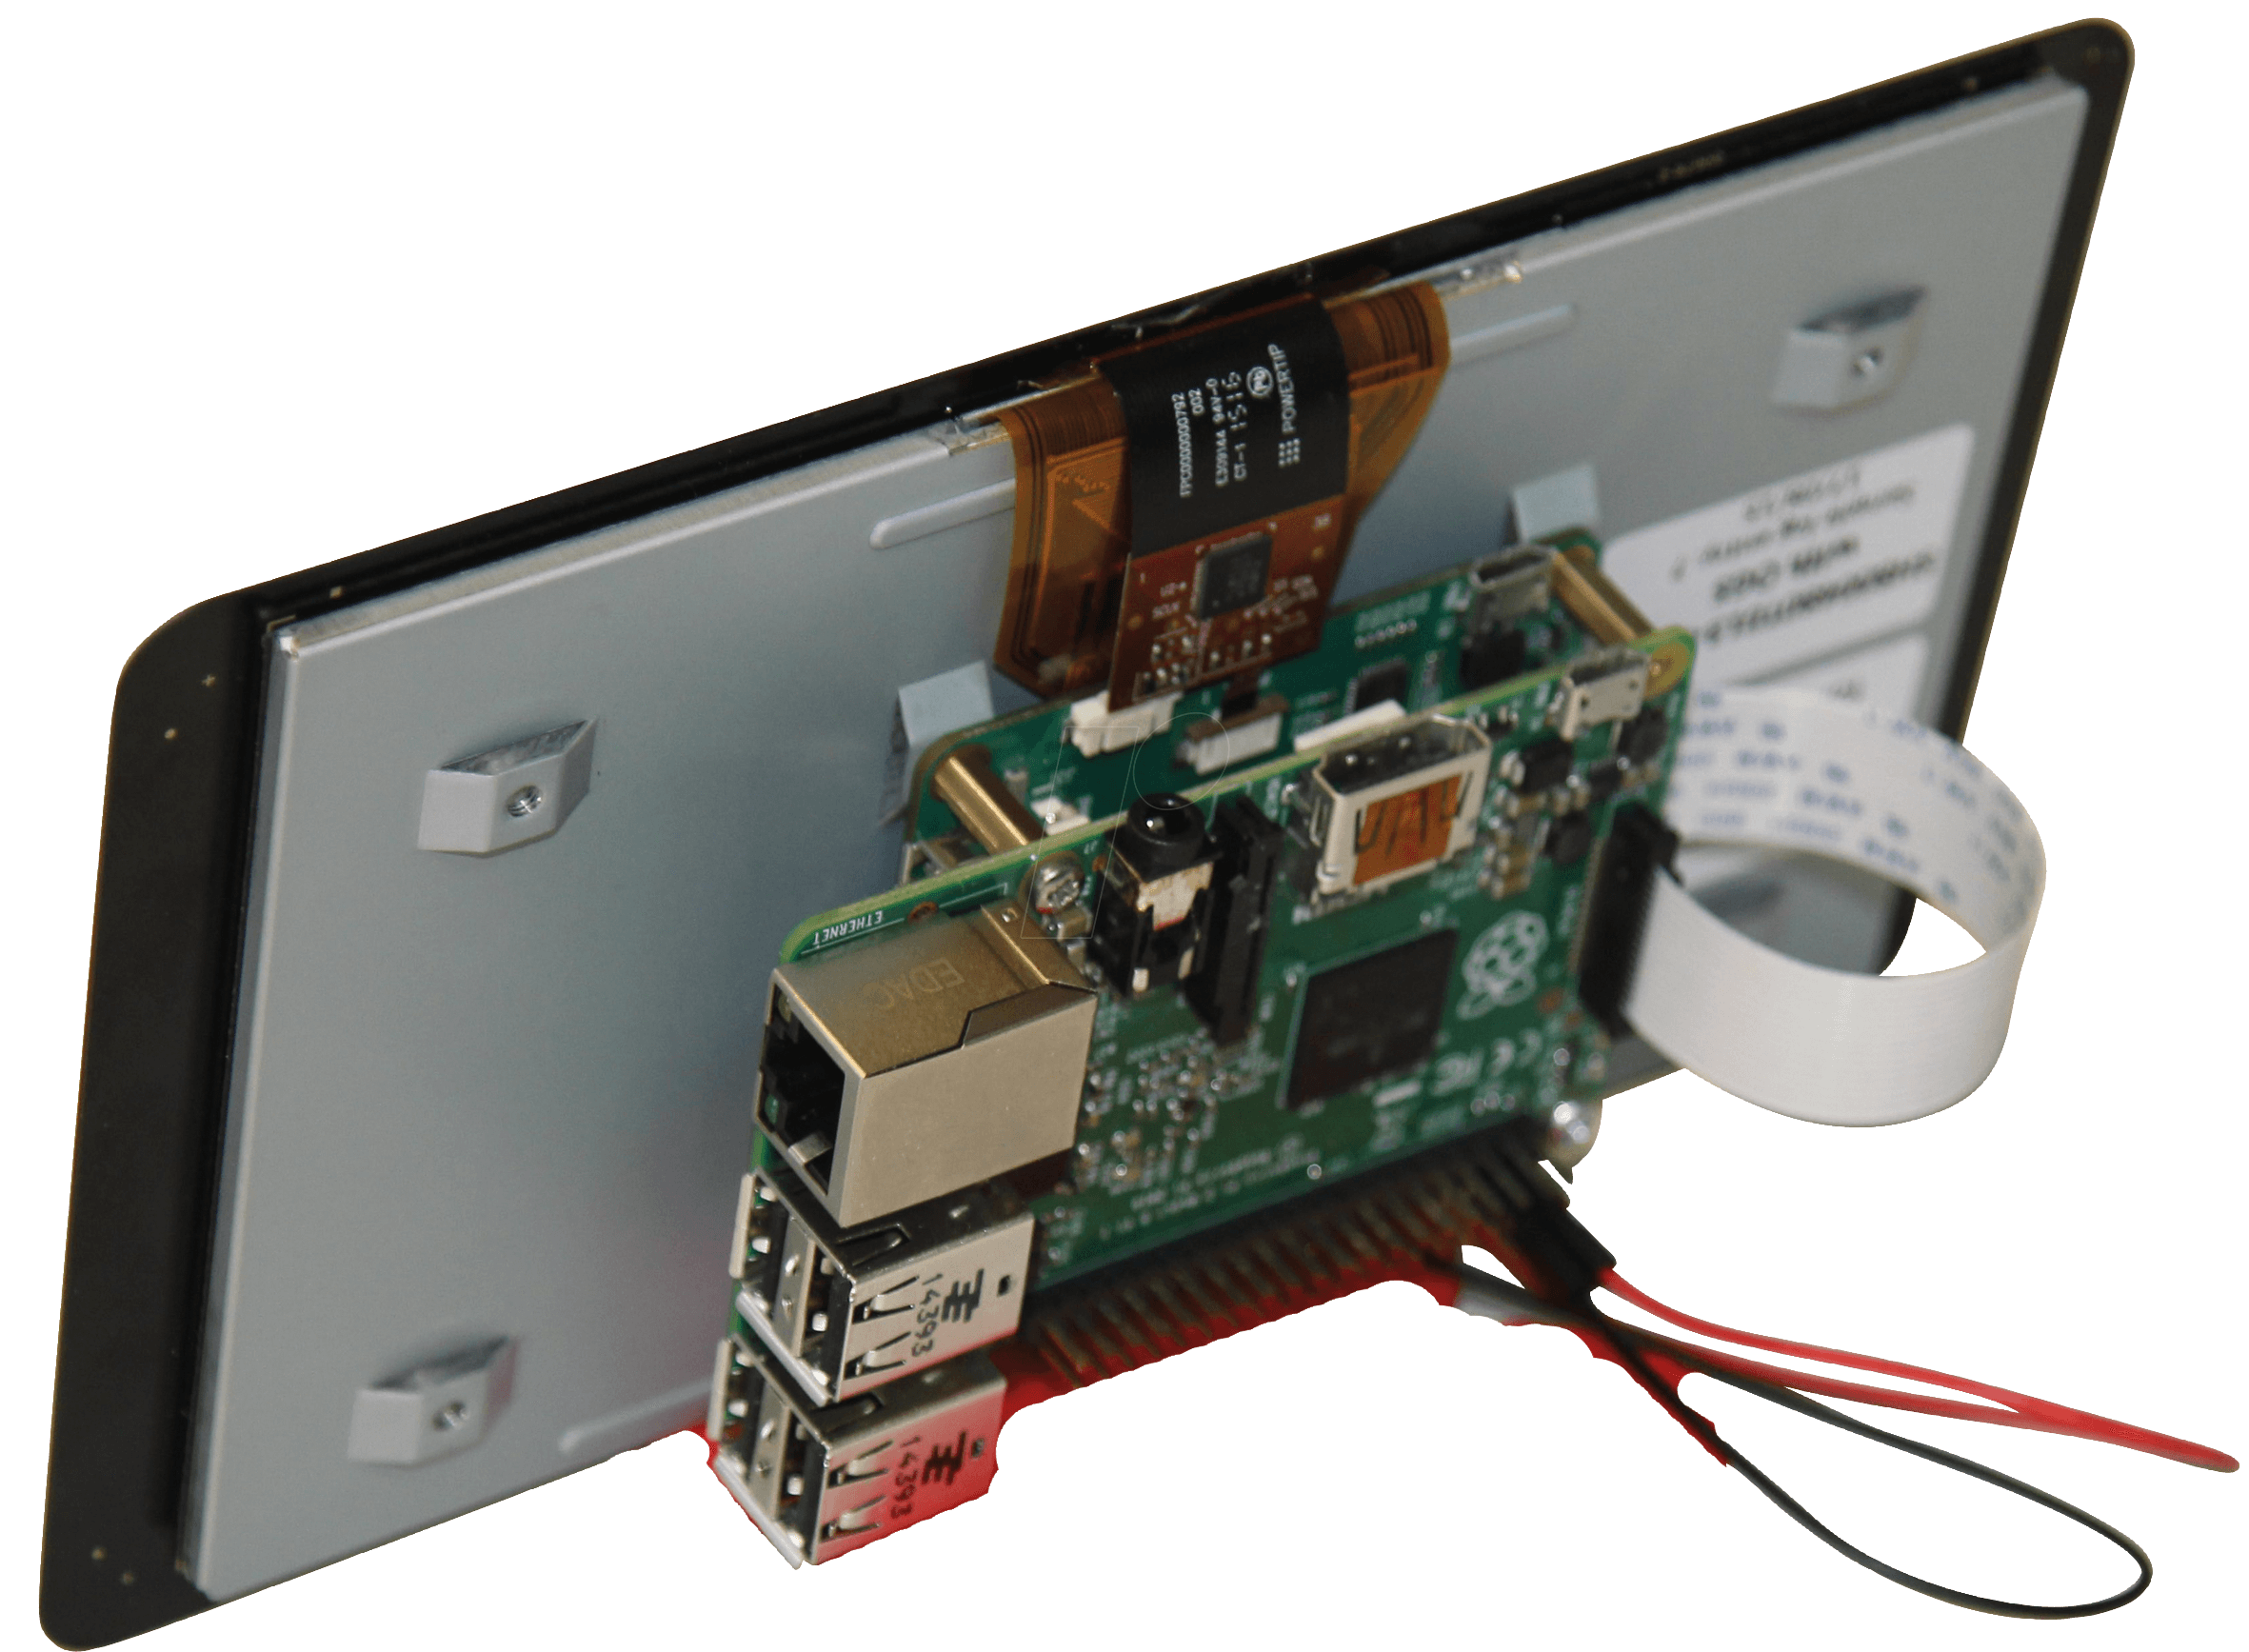
\includegraphics[width=0.8\columnwidth]{images/applicabilita/RPiwithDisplay.png}
    \end{center}
    \caption{Raspberry Pi con display originale}
    \label{fig:raspi-with-display}
\end{figure}
Creando un setup con quest'ultimo, altoparlanti, microfono ed un display da 7", la spesa sarebbe di circa \textbf{cento euro alla data odierna}. Questo costo è senz'altro più basso di tanti dispositivi enterprise proposti ogni giorno agli ospedali, oltre a garantire \textbf{tutela dei dati}, \textbf{apertura delle logiche} di funzionamento (open source), \textbf{semplicità} di utilizzo. Un altro dispositivo molto interessante per questo progetto è il \textbf{Mycroft Mark II}, sviluppato direttamente dai creatori dell'assistente vocale, integrante tecnologie di cancellazione del rumore, un display per l'interfaccia grafica, altoparlanti e kernel Linux, con possibilità di accesso SSH per la configurazione e la codifica di nuove skills. Quest'ultimo costerà, al suo lancio, poco più di cento euro, e rappresenta l'alternativa perfetta ad un sistema autocostruito, probabilmente troppo sperimentale per un ospedale. La \textbf{privacy} è in ogni caso \textbf{garantita} dal team.
\begin{figure}[H]
    \begin{center}
        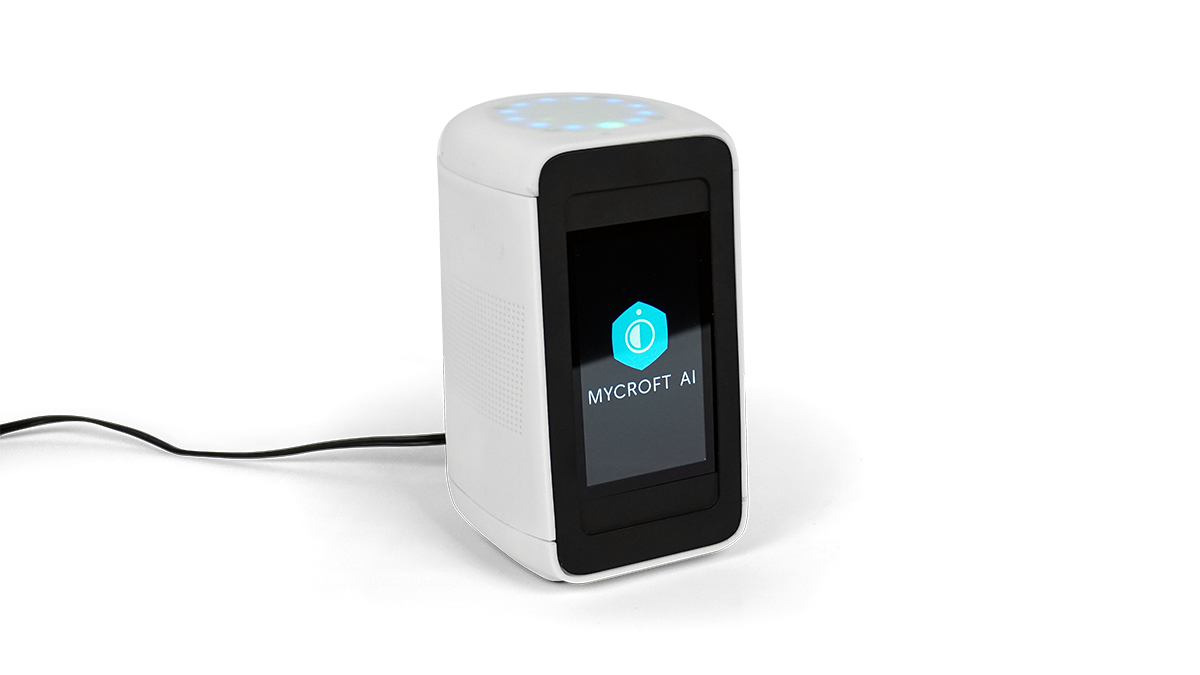
\includegraphics[width=0.8\columnwidth]{images/applicabilita/Mark_II.png}
    \end{center}
    \caption{Mycroft Mark II}
    \label{fig:mark-II}
\end{figure}
\begin{center}
    \textit{The Mycroft Mark II smart speaker is an open solution for individuals and companies who want to deploy voice technology, but don’t want to be in orbit around Silicon Valley.  Our technology can be run on premises and provides a great voice experience without sacrificing privacy.}
\end{center}

\chapter{Conclusioni}
\label{chap:conclusioni}
La pandemia globale sviluppatasi nel corso dell'anno 2020 ha messo in luce come gli ospedali, negli ultimi anni, siano stati man mano dimenticati dalla politica e dai budget. Il più recente rapporto sullo stato del SSN,\textit{Annuario Statistico del Servizio Sanitario Nazionale}, è stato pubblicato a settembre 2019 e contiene dati riferiti al 2017.
Tra il 1998 e il 2017, il numero degli istituti di cura è diminuito di circa 400 unità su 1400. Il numero di posti letto, passato da 311 mila a 191 mila. La spesa pubblica per la sanità, è però costantemente aumentata, pasando da meno di 60 miliardi di euro, a più di 112. \cite{article:tagli-ospedali} Pare ovvia la necessità di una riforma del servizio sanitario pubblico, e la tecnologia potrebbe, in questa, assumere un ruolo chiave. L'utilizzo di strumenti informatici allo stato dell'arte in ambito ospedaliero ridurrebbe le spese, migliorerebbe le performance, e permetterebbe di curare più pazienti, in modo migliore.
Spesso la popolazione guarda verso la tecnologia con malfidenza: per questo, la necessità è rendere questo passaggio il più impercettibile ed \textit{umano} possibile. Strumenti come gli assistenti vocali, le app mobili, la realtà aumentata possono contribuire ad appiattire il \textit{digital divide}, rendendo i servizi fruibili anche alle fasce d'età più restie a questi avanzamenti della società, spesso le più frequenti utilizzatrici dei servizi sanitari.
La ridotta complessità di questo progetto è la prova che spesso le migliorie necessarie sono ben più vicine di quanto sembrino.
Il lavoro è \textit{diviso} in due parti: una basata sulle reti neurali di Padatious, allenate con alcune frasi per sintomo, ed una basata sulla libreria fastai, allenata con un dataset apposito. Ognuna delle due ha, senz'altro, possibilità di evoluzione: il miglior risultato si otterrebbe accorpandole ed affidandosi totalmente ad un classificatore esterno a Mycroft. Questo richiederebbe però un dataset di training molto più completo e numeroso, e per questo la decisione di affidarsi a \textbf{due livelli} di skills si è rivelata la più affidabile. Ciò non toglie che, con lo sviluppo di nuovi dataset nel futuro, sarà un giorno possibile definire un progetto come questo ancora più semplicemente.
Inoltre, la possibilità di installare questo assistente vocale su dispositivi a basso costo piuttosto che appositi totem high-end, rende abbordabile il passaggio ad un pre-triage automatizzato a quasi tutti gli ospedali e cliniche italiani.
Tutto il codice scritto per la tesi è open source con licenza GPL-3.0. Il codice stesso del documento \LaTeX di questa tesi è open source.
Questo permette l'analisi, da parte di chiunque, del codice per il riscontro di bugs e problemi. Ne permette l'espansione, l'utilizzo gratuito, la sperimentazione da parte dei programmatori e degli ospedali. Infine, è corretto e necessario:
\begin{center}
    la libertà, delle persone come del software, è \textbf{l'unica via per il progresso.}
\end{center}


%%%%%%%%%%%%%%%%%%%%%%%%%%%%%%%%%%%%%%%%%%%%%%%%%%%%%%%%%%%%%%%

% BIBLIOGRAFIA
\phantomsection
\addcontentsline{toc}{chapter}{\refname}
\nocite{*}
\printbibliography

\end{document}
